\question{Ортогональность вектора подпространству. Ортогональное дополнение. Теорема Пифагора.}

\begin{definition}\label{ort-subspace-def}
  Пусть дано Евклидово пространство \(E^{n}\).
  Элемент \(h \in E^{n}\) называется ортогональным (перпендикулярным)
  подпространству \(G \subset E^{n}\), если \(\forall x \in G \colon h \bot x\).
\end{definition}

\begin{corollary}
  Выделим в подпространстве \(G\) базис
  \(\Basis = \{\basis_{1}, \dotsc, \basis_{k} \}\).
  Если \(h \bot e_{i} \forall \basis_{i} \in \Basis\), то \(h \bot G\).
\end{corollary}
\begin{proof}
  Любой элемент \(x \in G\) можно представить в виде
  \(x = \sum_{i = 1}^{k} \lambda_{i} \basis_{i}\).
  Рассмотрим скалярное произведение \((h, x)\).
  По свойствам линейности разложим его на
  \(\sum_{i = 1}^{k} \lambda_{i} (h, \basis_{i})\).
  Т.к. \(h\) ортогонален каждому из базисных векторов, то полученная сумма
  будет равна нулю, значит \(h\) ортогонален любому \(x \in G\).
\end{proof}

\begin{definition}\label{ort-compl-def}
  Пусть дано Евклидово пространство \(E^{n}\).
  Ортогональным дополнением \(F\) к подпространству
  \(G \subset E^{n}\) называется совокупность векторов \(h \bot G\).
\end{definition}

\begin{remark}
  Из определения \ref{ort-subspace-def} следует, что \(F\) также является
  подпространством \(E^{n}\).
\end{remark}

\begin{theorem}
  Евклидово пространство \(E^{n}\) является прямой суммой подпространства
  \(F \subset E^{n}\) и его ортогонального \(G = F^{\bot}\).
  
  \begin{lequation}{ort-compl-sum-thr}
    E^{n} = F \oplus F^{\bot}
  \end{lequation}
\end{theorem}
\begin{proof}
  В Евклидовом пространстве \(E^{n}\) выделим базис, после чего разложим
  произвольный элемент пространства \(x \in E^{n}\) по этому базису:

  \begin{lequation}{ort-compl-sum-thr-proof}
    \Basis = \{
      \underbrace{\basis_{1}, \dots, \basis_{k}}_{\text{Базис } G},
      \basis_{k + 1}, \dots \basis_{n}
    \} \\
    x
    = \underbrace{x_{1} \basis_{1} + \dots + x_{k} \basis_{k}}_{\overline{x}}
    + \underbrace{x_{k + 1} \basis_{k + 1} + \dots + x_{n} \basis_{n}}_{\hat{x}}
    = \overline{x} + \hat{x}
  \end{lequation}

  $\forall e_1, \, \dots, \, e_k$ ортогонален $\forall e_{k+1}, \, \dots, \, e_n$, то есть ортогонален $\hat{x}$ 
  как линейной комбинации.

  $\hat{x} \perp e_1, \, \dots, \, e_k$, то есть $\hat{x} \perp \overline{x} \implies \hat{x} \perp G$. Множество $\hat{x}$ составляет $F$.
\end{proof}

\begin{theorem}\label{pifagor-thr}
  \textbf{Пифагора}:

  \begin{figure}[H]
  \begin{center}
    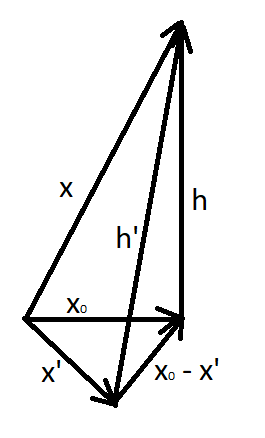
\includegraphics[width=100pt]{LA/Pifagor.png}
  \end{center}
  \label{ris:Pifagor}
  \end{figure}
  
  \begin{lequation}
    |||h'|| > ||h|| \, \text{(длина наклонной больше длины перпендикуляра)}\\
    ||x-x'||^2 = ||\underbrace{x - x_0}_{n} + x_0 - x'||^2 = \, \text{(Пифагор)} \, ||x-x_0||^2 + ||x_0-x'||^2 > ||x-x_0||^2 \, (\neq, \text{т.к. } x' \neq x_0)
  \end{lequation}
\end{theorem}